\chapter{Разработка алгоритма для игры NetHack с применением машинного обучения с подкреплением}\label{ch:ch3}

\section{NetHack - одна из самых сложных игр для RL}

Игра NetHack одна из старейших и наиболее популярных rouge-подобных игр. Первая версия игры появилась в 1987 году, а последняя вышла в 2020. В начале игры, герой оказывается в подземелье в котором он должен найти амулет Вендора. Для этого герой должен пройти более чем 50 процедурно генерируемых уровней. Игра имеет текстовый интерфейс представленный на рис.~\ref{fig:nethack_map}. В центре с помощью ascii символов изображается подземелье, сверху появляется текстовое сообщение описывающее положение в игре, а снизу содержится информация о состоянии героя. 

\begin{figure}[ht]
\centerfloat{
        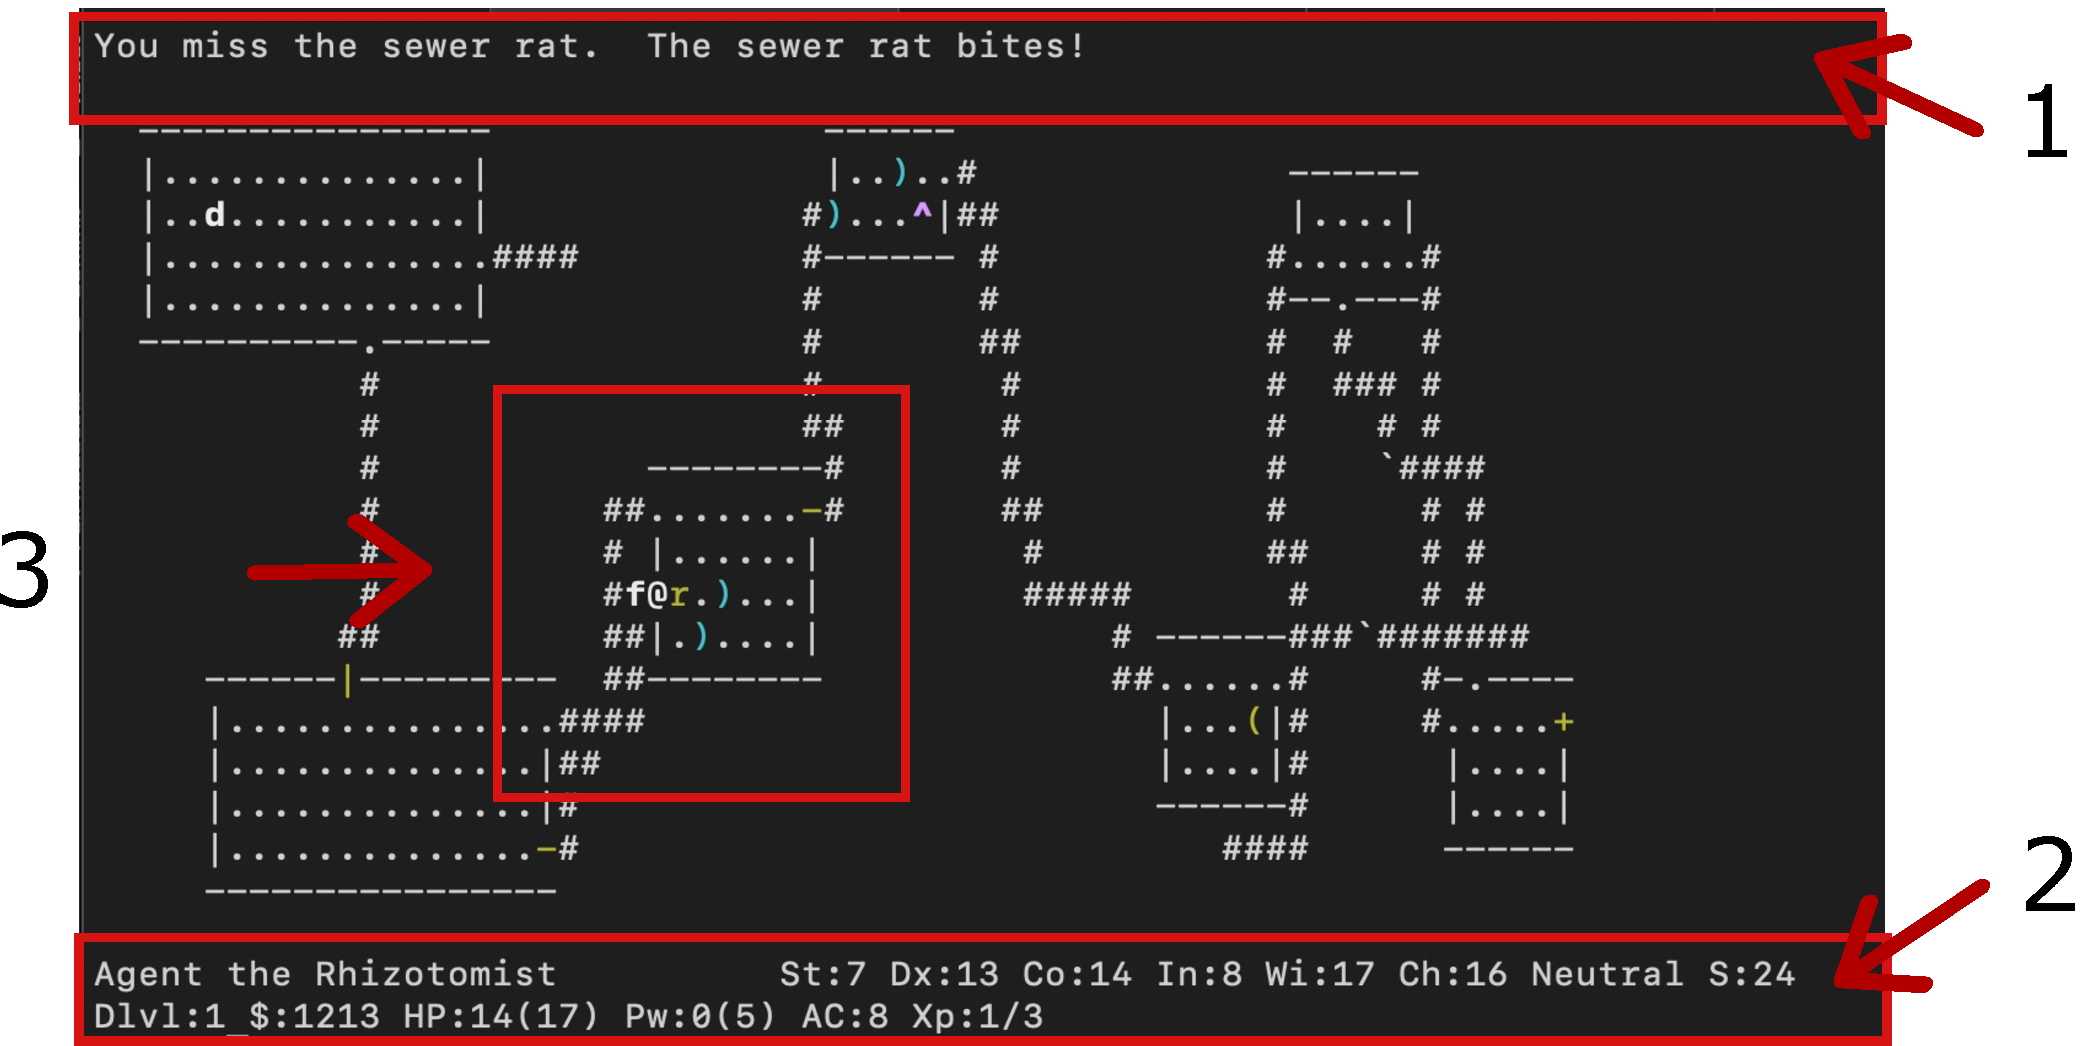
\includegraphics[width=0.85\textwidth]{images/nethack_map_view.pdf}
}
\caption{Интерфейс игры NetHack. (1) текстовое сообщение описывающее текущее событие, (2) статистика агента (здоровье, золото, сила, и др.) (3) окно центрированное возле текущего положения агента (@).}
    \label{fig:nethack_map}
\end{figure}

Несмотря на простой интерфейс NetHack ставит перед игроком сложные задачи. Далее опишем основные сложности которые делают NetHack серьезным испытанием как для человека, так и для RL агента.

\begin{itemize}
    \item \textbf{Процедурная генерация среды.} Многие компоненты игры являются процедурно генерируемыми и имеют случайную динамику. Например, точное положение интересующих объектов таких как расположение предметов, монстров, еды и также структура подземелий генерируются случайным образом. Использование процедурной генерации уровней приводит к тому, что агент практически никогда не попадет в точно такую же ситуацию в которой он был в прошлом. При обучении RL агентов это приводит к фундаментальной проблеме с количеством данных необходимых для обучения и позволяет оценить способность агента обобщать свою текущую стратегию на новые задачи. Также в игре NetHack не работают методы исследования среды Go-Explore \cite{ecoffet2019, ecoffet2021} основанные на стратегии, умеющей возвращаться в ранее посещенные состояния которые в других задачах показывают наилучшие результаты. Кроме того, состояние в игре NetHack состоит из сотен возможных символов, что приводит к огромному количеству возможных состояний. Более того, в игре NetHack у героя могут быть различные роли (например, монах, валькирия, волшебник, турист), расы (человек, эльф, гном, орк) и различные начальный набор предметов. 
    \item \textbf{NetHack -- очень длинная игра.} Эксперту для прохождения игры NetHack требуются десятки тысяч ходов. У среднего игрока прохождение игры может занять многие дни и более сотни тысяч ходов. По сравнению с другими тестовыми задачами для RL агентов такими как  StarCraft и Dota 2, эпизоды в NetHack на один или два порядка длиннее и сильно зависят от текущей стратегии агента. 
    \item \textbf{Много модальные наблюдения.} Как показано на рис.~\ref{fig:nethack_map} в текущее состояние агента входит графическое изображение карты и его положение на ней; сообщение на естественном языке описывающее текущее событие; числовые признаки описывающие состояние агента; категориальные признаки описывающие имеющиеся в распоряжении у агента предметы и особенные свойства агента. 
\end{itemize}

Также сложность игры подчеркивает то, что для NetHack существует обширное описание \cite{nethack_wiki} возможных стратегий поведения созданное активными игроками которое может быть использовано для обучения RL агентов. Кроме того, существует репозиторий с большим количеством записей реальных игроков \cite{alt} который может быть использован для обучения агента имитировать их стратегии. Таким образом NetHack ставит уникальные задачи для исследований в области применения RL агентов. 

\subsection{NLE - среда основанная на игре NetHack}
В работе \cite{nethack} авторами для игры NetHack была разработана среда NLE для обучения RL агентов на основе версии NetHack 3.6.6. Среда NLE удовлетворяет gym интерфейсу \cite{brockman2016openai} и позволяет обучать RL агентов в игре NetHack. Важной особенностью NLE является то, что она практически не ограничивает возможностей агента в игре и он способен совершать такие же действия, как и человек использующий стандартный интерфйес. 

\paragraph{Пространство состояний.}
Пространство наблюдений состоит из глифов (уникальный идентификатор объекта в игре), символов и их цветов (сюръективное отображение глифов в текстовом терминале),  информации о текущем состоянии игрока, текстового сообщения на естественном языке, глифов соответствующих объектам находящимся в инвентаре, текстовых описаний объектов из инвентаря, символов используемых для отображения объектов из инвентаря в терминале и классов объектов из инвентаря. Набор из глифов, символов и их цветов описывают двумерное символьное представление подземелья изображенного на рис.~\ref{fig:nethack_map}. Информация о текущем состоянии игрока содержит его координаты $x,y$ в подземелье,  очки здоровья, силу, ловкость, уровень голода и другие характеристики. Текстовое сообщение содержит текст показываемый на данном шаге игроку. 

\paragraph{Пространство действий.} Пространство действий состоит из 113 дискретных действий, соответствующим действиям которые может совершать человек в игре NetHack. Из них 16 действий соответствуют перемещениям агента, а оставшиеся 97 --- командам. Агент может перемещаться в восьми направлениях на один шаг или до тех пор, пока  не столкнется с каким либо предметом. Оставшиеся 97 команд включают в себя такие команды как есть, открывать, читать, молиться и многие другие.

\paragraph{Награда.}
Агент получает награду напрямую из игры NetHack. Награду можно получать за различные действия, но наиболее часто она дается за победу над монстрами. Более детально награды перечислены на wiki странице \cite{nethack_wiki}. 

\paragraph{Эпизод.}
Длительность эпизода ограничена $10^7$ шагов. В начале каждого эпизода процедурно генерируется подземелье, и случайным образом выбирается раса и класс героя. Эпизод всегда начинается с первого уровня подземелья. 


\section{Декомпозиция игры NetHack на подзадачи}

Один из главных вызовов среды NLE для методов обучения с подкреплением состоит в том, что пространство действий сложно исследовать методом проб и ошибок:

\begin{itemize}
    \itemВ определенных состояниях среды действия не приводят ни к какому результату: нет еды, чтобы съесть; нет оружия, чтобы взять его в руку; нет рядом двери которую можно открыть. RL агенту для того, чтобы установить взаимосвязь между состоянием и действием нужно попробовать несколько раз выполнить каждое действие в каждом из состояний, что приводит экспоненциальному росту времени обучения. 
    \itemСледующий вызов состоит в том, что часть осмысленными являются не сами действия, а их последовательности. Например, для того чтобы написать слово ``Elbereth'' которое может защитить агента от нападения требуется последовательно выполнить одиннадцать действий. Это еще увеличивает размерность пространства для поиска оптимальных действий. 
    \itemТретий вызов заключается в том, что значение действий предоставляемых средой NLE также зависят от текущего состояния среды. Например, действие ``y'' в зависимости от контекста может означать как шаг на одну клетку вправо и вверх, указание для атаки, ответ ``да'' на вопрос, часть команды ``\#pray''.
\end{itemize}

Данная задача имеет иерархическую структуру которую можно использовать для упрощения обучения RL агента. Для этого мы реализовали обработку состояний поступающих от среды NLE. Обработка реализована в классе RLWrapper и включает в себя:

\begin{itemize}
    \item обработку текстовых сообщений
    \item нахождение монстров, дверей и предметов на карте
    \item управление инвентарем: определение ожидаемого урона, и количества оружия
    \item определение специфичных способностей героя
    \item преобразование высокоуровневых действий агента в низкоуровневые действия среды
\end{itemize}


\begin{figure}[ht]
\centerfloat{
        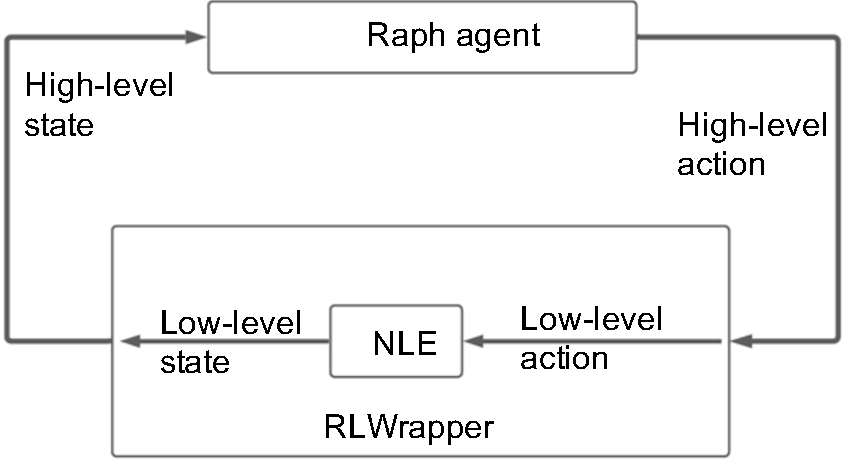
\includegraphics[width=0.75\textwidth]{images/raph_wrapper.pdf}
}
\caption{Схема взаимодействия RAPH агента со средой NLE.}
    \label{fig:raph_nle}
\end{figure}

Схематически взаимодействие RL агента и среды изображено на рис.~\ref{fig:raph_nle}. Для упрощения процесса обучения нами был выбран гибридный подход совмещающий обучение RL агента с экспертными стратегиями выполняющимися в соответствии с заданными приоритетами. Экспертные стратегии выполняются внутри класса RLWrapper, и их выполнение представляет собой один шаг среды с точки зрения RL агента. 

\section{Обучение иерархического агента совмещающего обучение с подкреплением и алгоритмический подход}

Мы применили иерархический подход для задания стратегии агента. Для этого с использованием экспертных знаний мы реализовали элементарные стратегии для определенных действий таких как еда, исследование подземелья, открытие дверей, поиск спрятанных предметов, молитва, взятие полезных предметов, атака близких и далеких монстров. Данный подход похож на систему опционов предложенною Р. Саттоном в работе \cite{Sutton1999}, в которой стратегия верхнего уровня управляет выполнением стратегий нижнего уровня. Данный подход позволил нам построить гибридный нейро-алгоритмический метод, в котором часть способностей обучается, а часть задается экспертно. В нашей задаче мы использовали упрощенную постановку в которой стратегия верхнего уровня задается алгоритмически и вызывает первую подходящую из стратегий нижнего уровня упорядоченных экспертным образом. 

При реализации большинства из экспертных действий используется алгоритм нахождения кротчайшего пути в графе для навигации к нужному объекту и затем выполняется соответствущее ему действие. В общей сложности нами было реализовано $12$ экспертных стратегий которые занимали 85\% от общего числа шагов, но приносили только 1\% от общей награды. Одной из наиболее важных способностей агента в среде NetHack является стратегия сражения с монстрами так как именно они приносят основную часть награды. Сражение с монстрами требует сложной стратегии которая бы учитывала топологию окружающую агента и выбор подходящего действия: приблизиться, обойти, не быть окруженным монстрами, использовать ближнюю или дальнюю атаку, восстановить здоровье, или пропустить ход. Поэтому для сражения с монстрами мы обучали RL агента. Обученный RL агент взаимодействовал со средой только в 15\% шагов, но получал 99\% суммарной награды. 

\paragraph{Пространство действий.} Пространство действий для RL агента состоит из 19 действий:
\begin{itemize}
    \item шаг или ближняя атака (x8 направлений)
    \item дальняя атака (x8 направлений)
    \item пропуск хода
    \item заклинание Elbereth
    \item молитва
\end{itemize}

\paragraph{Пространство наблюдений.} Пространство наблюдений включает в себя часть карты подземелья размером 9x9 символов центрированную по положению агента, информацию о герое и его вооружении, и маску допустимых действий. 

\paragraph{Передача управления.}
Передача управления к RL агенту происходит в случае если монстр находится на расстоянии менее пяти шагов от агента. Остальные шаги в которых управление переходит к экспертным стратегиям пропускаются RL агентом. 


\paragraph{Архитектура нейронной сети и алгоритм обучения RL агента.} При обучении RL агента использовался алгоритм impala \cite{impala} c параметрами аналогичными использованным работе \cite{kuettler2020nethack}. Архитектура нейронной сети актора представлена на рис.~\ref{fig:raph_arch}. В ней для преобразования двумерной карты подземелья используется двухслойная сверточная нейронная сеть, а для кодирования остальной информации двухслойный перцептрон. Получившиеся латентные представления объединялись вместе и преобразовались с помощью еще одного двухслойного перцептрона. Для того чтобы агент не мог совершать недоступные действия перед вычислением вероятностей операцией softmax соответствующие им компоненты устанавливались равными $-10^{10}$. 

\begin{figure}[ht]
\centerfloat{
        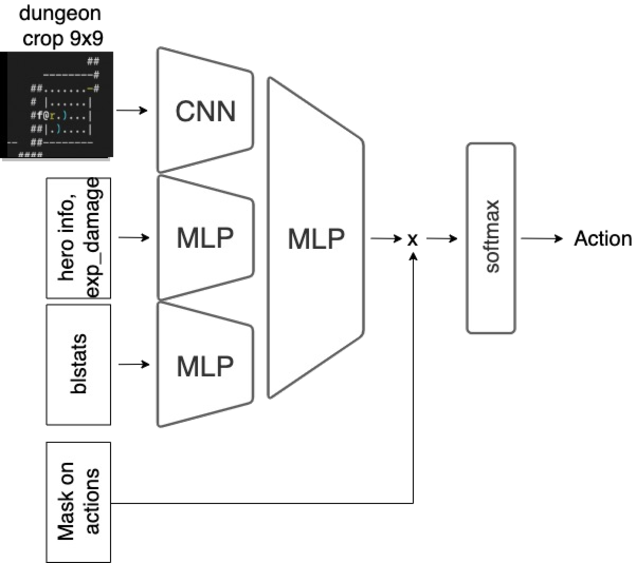
\includegraphics[width=0.75\textwidth]{images/raph_arch.pdf}
}
\caption{Архитектура нейронной сети актора RAPH агента в среде NetHack.}
    \label{fig:raph_arch}
\end{figure}

Рассмотрим алгоритм работы агента~\ref{alg:raph}. В первую очередь обрабатываются текстовые сообщения от среды с помощью регулярных выражений. Далее мы обрабатываем обновляем представление подземелья и извлекаем признаки необходимые для работы агента. Затем в зависимости от того, есть ли сейчас монстр в области видимости агента или нет мы выбираем действия или с помощью RL агента или из одной из экспертных стратегий.


\begin{algorithm}[H]
\SetKwComment{Comment}{/* }{ */}
\SetKw{Continue}{continue}
\caption{RAPH agent}\label{alg:raph}
\KwData{view\_distance, agent, hard\_coded\_skills}
$state, done \gets env.reset(), False$\;

\While{not done}{
  action\_queue = parse\_message(state)\;

  \If{action\_queue} {
   state, reward, done, info = env.step(action\_queue)\Comment*[r]{We have a prompt to response}
   \Continue
  }

  monster\_distance, preprocessed\_state = parse\_dungeon(state)\;
  \eIf{monster\_distance \textless view\_distance}{
    action\_queue = agent.act(preprocessed\_state)\;
  }{
    action\_queue = first\_fit(hard\_coded\_skills, preprocessed\_state)\Comment*[r]{Select non-rl action on first-fit basis}
  }
  state, reward, done, info = env.step(action\_queue)\;
}
\end{algorithm}

\paragraph{Анализ качества работы агента}

На рис.~\ref{fig:raph_train} показана средняя награда получаемая агентом в зависимости от числа шагов обучения. Видно, что благодаря экспертным стратегиям даже не обученный иерархический агент работает лучше, чем агент не использующий иерархию. Это происходит из-за того, что он умеет достаточно хорошо исследовать среду и реже умирает от голода. Обученный агент использует действия в следующей пропорции: 

\begin{itemize}
    \item ближняя атака 66\%
    \item дальняя атака 21.6\%
    \item пропуск хода 11\%
    \item ``Elbereth'' 0.3\%
    \item молитва 0.1\%
\end{itemize}


\begin{figure}[ht]
\centerfloat{
        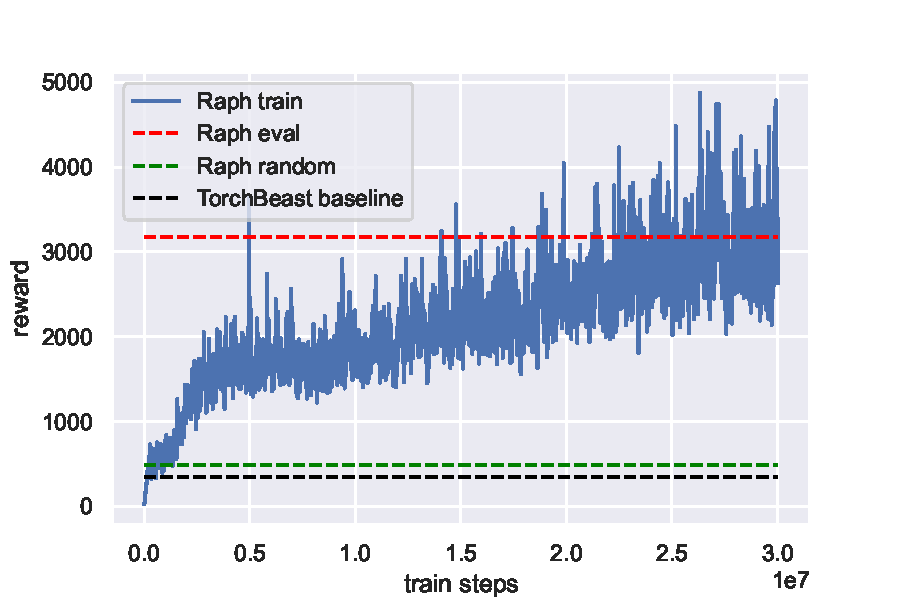
\includegraphics[width=0.95\textwidth]{images/raph_train.pdf}
}
\caption{Экспоненциальное скользящее среднее суммарной награды получаемой агентом в зависимости от количества шагов обучения. Красным цветом показано итоговое качество работы агента. Зеленым цветом показано качество работы не обученного агента. Черным цветом показано качество работы базового агента не использующего иерархию.}
    \label{fig:raph_train}
\end{figure}


В таблице~\ref{tab:raph_analize} представлена зависимость медианной награды получаемой агентом от его класса. Видно, что наибольшую награду агент получает при игре за такие классы как barbarian и samurai которые достаточно сильны в ближнем бою. Это означает, что агент в основном использует довольно простые стратегии борьбы с монстрами которые хорошо работают на изначально сильных персонажах, но не очень подходят для слабых. 

\begin{table} [htbp]
    \centering
    \begin{threeparttable}
        \caption{Медианная награда получаемая агентом в зависимости от его роли.}\label{tab:raph_analize}
        \begin{tabular}{| p{8cm} || p{8cm} |}
            \hline
            \hline
            класс & награда \\
            \hline
            archeologist & 1881 \\
            barbarian & 4757 \\
            caveman & 708 \\
            healer & 1057 \\
            knight & 2697 \\
            monk & 1727 \\
            priest & 629 \\
            rogue & 2694 \\
            samurai & 3604 \\
            tourist & 1108 \\
            valkyrie & 4094 \\
            wizard & 1041 \\
            \hline
            \hline
        \end{tabular}
    \end{threeparttable}
\end{table}

\section{Выводы}

В рамках данной работы нами был разработан гибридный нейро-символьный метод для управления
виртуальным агентом в среде NetHack. В разработанном методе RL агент решает одну из наиболее сложных задач возникающих в среде NetHack --- сражение с монстрами. Для остальных задач используются экспертные стратегии. В результате тестирования было показано, что данный подход позволяет достичь хороших результатов и значительно превзойти базового агента основанного только на обучении с подкреплением. В соревновании по игре NetHack проводимом в рамках конференции NeurIPS 2021 разработанный нами агент занял первое место среди агентов использующих в своей работе нейронные сети. В дальнейшем добавление новых экспертных стратегий и улучшение их приоритизации может существенно улучшить качество работы агента. 


\clearpage
